\documentclass[../Skript.tex]{subfiles}
\graphicspath{{\subfix{../images/}}}
\begin{document}

Aufgabe der Interpolation ist es, diskrete Datenwerte durch eine Kontinuierliche Funktion darzustellen.
\begin{center}
    BILD!
\end{center}
Dabei sollen die Datenpunkte $(x_i,y_i), i=1,...,n$ exakt durch eine ''interpolierende'' Funktion $f:I\subset\R \to\R$ mit 
$f(x_i)=y_i$ dargestellt werden. Vorraussetzung: $x_i$ paarweise verschieden!\\\\
Idee dahinter: Datenpunkte sind nur Punktauswertungen einer ''glatten'' Funktion, die durch $f$ approximiert werden soll. 
Nach der interpolierenden Funktion $f$ wird üblicherweise in einem ''einfachen'' Funktionenraum gesucht. Z.B. Polynome 
Trigonometrische Funktionen,..., evntuell nur stückweise definierte aber insgesamt glatte Funktionen.\\\\
Zusätzlich zu Funktionen $f(x_i)=y_i$ können auch evntuell Ableitungen $f'(x_i)=z_i$ vorgegeben sein.\\\\
Das ganze funktioniert ähnlich auch bei Daten und Funktionen über mehrdimensionalen Gebieten, z.B. Rekonstruktion von $2$D-
Flächen in $3$D (Computergraik, CAD) 

\section{Polynominterpolation}
Ein einfacher Ansatz: Interpolation durch Polynome. 
Ein Polynom vom Grad $n$ ist hier eine Funktion\\
\[p:\R \to \R , \ p(x)= a_0+a_1x+a_2x^2+\dots+a_nx^n\] mit reellen Koeffizienten \[a_0,\dots,a_n\in\R,\ a_n\neq 0 \leadsto 
\text{Grad } n\]
Es bildet
\[\mathbb{P}_n:=\{p(x)=a_0+a_1x+a_2x^2+\dots+a_nx^n \ \mid \ a_i\in\R ,\ i=0,\dots, n\}\] Die Menge der Polynome vom Grad 
$\leq n$\\
$\mathbb{P}_n$ bildet einen $\R$ Vektorraum, $$(p+q)(x):=p(x)+q(x), \ (\alpha p)(x):=\alpha p(x)\  \forall \alpha\in\R,\ 
p,q\in\bbP_n$$
Die ''Monome'' $\{1,x,x^2,\dots,x^n\}$ bilden eine Basis von $\mathbb{P}_n$, mit dim$(\mathbb{P}n)=n+1$.
\begin{definition}
    Die Aufgabe der Polynominterpolation besteht darin, zu $n+1$ paarweise verschiedenen Punkten $x_i, i=0,\dots, n$ 
    (''Stützstellen'', ''Knoten'') und gegebenen Knotenwerten $y_i, i=0, \dots, n$ ein Polynom $p\in\bbP$ zu bestimmen, mit 
    der Eigenschaft: \[p(x_i) = y_i, \ i=0,\dots,n\]
\end{definition}

\begin{theorem}
    Die Aufgabe der Polynominterpolation ist eindeutig lösbar, d.h. es gibt genau ein $p\in\bbP_n$,
    das die Bedingung erfüllt.    
\end{theorem}
\begin{proof}\hfill\\
\begin{enumerate}[(a)]
    \item Eindeutigkeit der Lösung:\\ angenommen $p\in\bbP_n$ und $q\in\bbP_n$ seien zwei Lösungen, $p(x_i)=y_i = 
    q(x_i)$.\newline Für die Differenz $p-q\in\bbP_n$ gilt dann: \newline
    $p-q$ hat $n+1$ Nullstellen in den $x_i, i=0,\dots, n$, aber ein $\Tilde{p}\in \bbP_n$ kann höchstens $n$ verschiedene 
    Nullstellen haben, oder es gilt $\Tilde{p}\equiv 0$ (z.B. über Satz von Rolle). Also ist $p\equiv q$, es gibt demnach 
    höchstens eine Lösung in $\bbP_n$ 

    \item Existenz einer Lösung:\\
    $p(x)= a_0+a_1x+a_2x^2+\dots+a_nx^n,\ p(x_i)=y_i, \ i=0,\dots,n$\\
    $\begin{pmatrix}
    1 & x_0 & x_0^2 & \cdots & x_0^n \\
    1 & x_1 & x_1^2 & \cdots & x_1n \\
    \vdots & \vdots & \vdots & \ddots & \vdots \\
    1 & x_n & x_n^2 & \cdots & x_n^n \\
    \end{pmatrix}
    \begin{pmatrix}
        a_o \\
        a_1 \\
        \vdots \\
        a_n
    \end{pmatrix} 
    =
    \begin{pmatrix}
        y_o \\
        y_1 \\
        \vdots \\
        y_n
    \end{pmatrix}$\\
    Bedingungen führen auf lineares Gleichungssystem und Matrix $V_n$ (Vandermonde-Matrix)\\
    Man kann zeigen: $$\det{V_n}=\dprod^n_{i=0}\dprod^n_{j=i+1} (x_j-x_i) \neq 0 $$falls alle $x_i$ paarweise verschieden 
    sind. Also ist das lineare Gleichungssystem eindeitig lösbar, wenn $\det{V_n}\neq 0$ bzw. wenn die Stützstellen paarweise verschieden sind. Zu beliebiger recher Seite 
    $(y_0,\dots,y_n)$ gibt es also Koeffizienten $(a_0,\dots,a_n)$ für ein interpolation Polynom.\\
\end{enumerate}
\end{proof}

Das Lineare Gleichungssystem liefert im Prinzip auch eine Berechnungsmethode, ist aber schlecht konditioniert, und die 
Lösung ist relativ aufwändig.

\subsection{Lagrange-Interpolation}\hfill\\
\subsubsection*{Idee} Wähle Basispolynome für $\bbP_n$ angepasst an die Stützstellen $x_i$, so dass das 
Interpolationspolynom damit aus den Werten $y_i$ leicht bestimmt werden kann. Man kann 
recht einfach Polynome $L_i^{(n)}\in\bbP_n$ konstruieren, die in genau einem Stützpunkt $x_i = 1$ sind und 
in allen anderen Stützpunkten = 0. $$L_i^{(n)}(x_i) = \left(\begin{cases}
    1& i=j\\ 0& \text{sonst}
\end{cases}\right) = \delta_{ij}$$
 $n$ Nullstellen $$x_j, j\neq i \implies L_i^{(n)} = \frac{\displaystyle\prod_{j\neq i}(x-x_j)}{\displaystyle\prod_{j\neq 
 i}(x_i-x_j)}$$
Diese $L_i^{(n)}, i=0, \dots, n$ heißen ''Lagrange-Basispolynome'' zu Stützstellen $x_0,\dots,x_n$.

Linear unabhängig: leicht zu sehen: Alle $L_j^{(n)}(x_i) = 0$. Anzahl ist gleich $\dim \bbP_n$

\begin{example} $n=1\  x_0,x_1$ \\
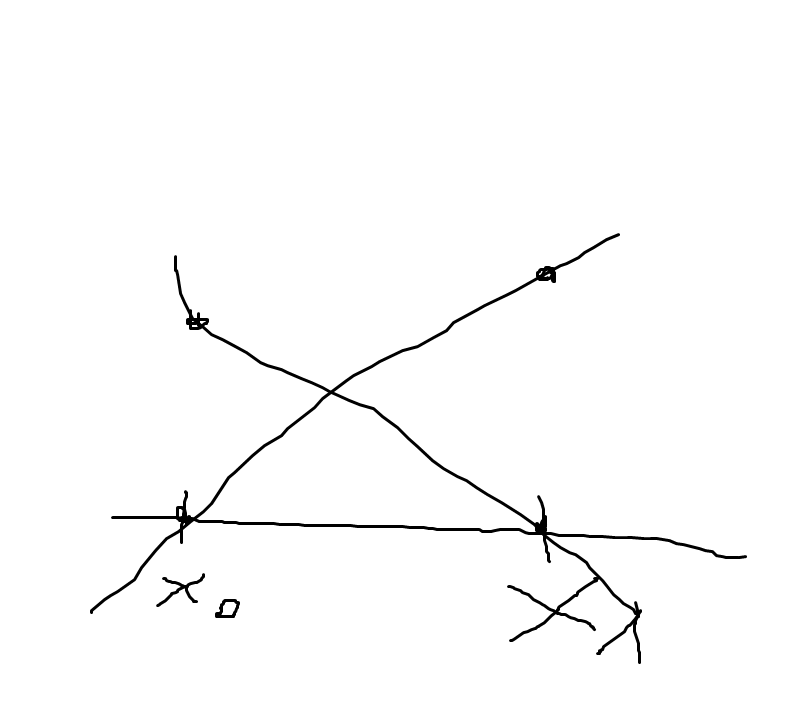
\includegraphics[width=45mm]{../Bilder/x_1_2.png}\\
$n=2$\\
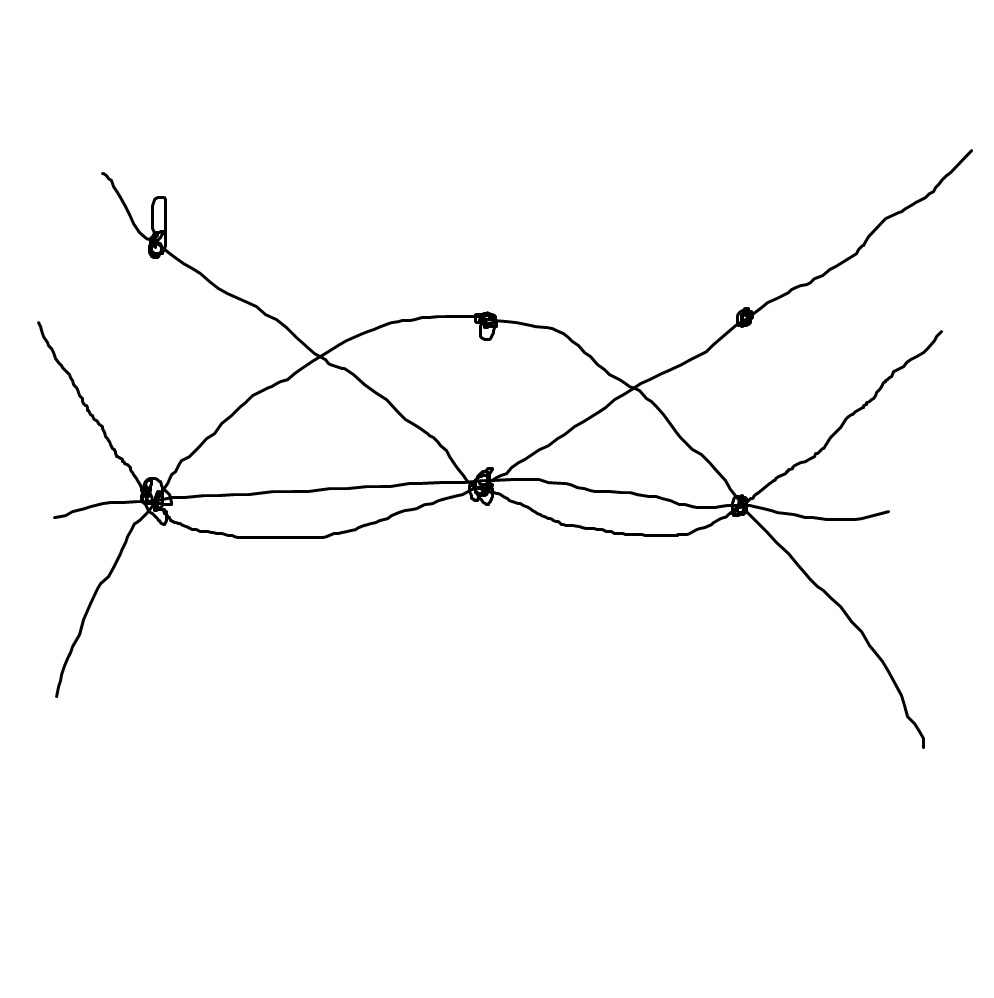
\includegraphics[width=45mm]{../Bilder/x_1_2_3.png}\\
\end{example}
\begin{remark}
auch in höheren Dimensionen, $\leadsto$ Numerik partieller Differentialgleichungen ''Finite Elemente Methode'' \\ 
\end{remark}


\begin{definition}
    Das Polynom $p(x)\coloneqq \dsum_{i=0}^n y_i\cdot L_i^{(n)}(x)$ heißt Lagrange-Interpolationpolynom
    zu den Stützstellen $x_0,\dots,x_n$ und Daten $y_0,\dots,y_n$.
\end{definition}
\subsubsection*{Vorteil:}
Für festes $n\in \N$ und Stützstellen $(x_0,\dots, x_n)$ relativ leicht zu berechnen, natürliche Darstellung des 
Interpolationpolynoms mit einfachen Koeffizienten
\subsubsection*{Nachteil:}
\begin{itemize}
    \item Für viele bzw eng beieinander liegende Stützstellen ist die Formel für $L_i^{(n)}$ relativ schlecht konditioniert 
    (Auslöschungseffekte)
    \item Will man weitere Stützstellen und Daten dazunehmen, muss komplett neu gerechnet werden
\end{itemize}
\subsection{Newton Darstellung}\hfill\\
Alternative Darstellung, auch an die Stützstellen angepasst.
Eine Polynombasis, die auch zu den Stützstellen passt, aber leicht erweiterbar ist: ''Newton-Basis''
\begin{align*}
    N_0(x) &\coloneqq 1 \text{ konstant}\\
    N_i(x) &\coloneqq \displaystyle\prod_{j=0}^{i-1}(x-x_j), \ i=1,\dots,n
\end{align*}
\[
    \text{Grad}(N_i) = i \implies (N_i) \text{ linear unabhängig},\ \lin{N_0,\dots,N_i} = \bbP_i, \text{ (Basis von }\bbP_i)
\]
Damit kann auch das Interpolationspolynom $p$, $p(x_i)=y_i, \ i=0,\dots,n$ in dieser Basis dargestellt werden, 
$p=\sum^n_{i=0}a_iN_i$\\
Koeffiziernten $a_i$
\begin{align*}
a_0&= y_0 &&\ \\
y_1&= p(x_1) =a_0+a_1(x_1-x_0)+0 \implies a_1=\frac{y_1-a_0}{x_1-x_0} \\
y_n&= p(x_n) =a_0+a_1(x_n-x_0)+a_2(x_n-x_0)(x_n-x_1)+\dots+ a_n(x_n-x_0)\dots(x_n-x_{n-1})\\ \implies a_n&= \frac{y_n-
\sum^{n-1}_{i=0}a_i\prod_{j<i}x_n-x_j}{\prod^{n-1}_{j=0}x_n-x_j} 
\end{align*}

\subsubsection*{Vorteil:}\hfill\\
\begin{itemize}
    \item Man kann beliebig zusätzliche Stützstellen dazunehmen, ohne bisherige Berechnung zu verwerfen
    \item Reihenfolge/Ordnung der Stützstellen beliebig
\end{itemize}
Einfacher Algorithmuns zur Berechnung der Koeffizienten: 
\begin{theorem}[Newton Darstellung mit dividierten Differenzen]
    Das Interpolationspolynom zu den Punkten $(x_i, y_i), i=0,\dots,n$ lässt sich bzgl. der Newton-Basis
    darstellen als \[
        p(x) = \dsum_{i=0}^n y[x_0, \dots, x_i]N_i(x)
    \]
    Dabei bezeichnen $y[x_0, \dots, x_i]$ die zu $(x_j, y_j)$ gehörenden ''dividerte Differenzen'', rekursiv 
    definiert als \[
    y[x_i] \coloneqq y_i, i=0\dots,n
    \]
    \[
    y[x_i, x_{i+1}, \dots, x_{i+k}] \coloneqq \frac{y[x_{i+1}, \dots, x_{i+k}] - y[x_i, \dots, x_{i+k-1}]}{x_{i+1} - x_i}, 
    \quad i=0, \dots, n, \midspace k=1, \dots, n-i
    \]
\end{theorem}

\begin{proof}\hfill\\
    Zu $i,n$ sei $P_{i,i+n}$ das Polynom, das $(x_i,y_i)\dots(x_{i+l},y_{i+k})$ interpoliert. $\implies \ p= P_{0,n}$ ist 
    gesucht.\\\\
    \emph{Behauptung.}:\(P_{i,i+k}(x)= y[x_i]+y[x_i,x_{i+1}](x-x_i)+\dots y[x_i,x_{i+k}](x-x_i)\dots (x-x_{i+k-1)} \)\\ \\
    Per induktion über $k$: $k=0 : \ P_{i,i}(x)=y_i=y[x_i]$ \\
    angenommen, es gilt für $k-1$.\\
    Es ist $$P_{i,i+k}=P_{i,i+k-1}+a(x-x_i)\dots(x-x_{i+k-1})$$ mit $a\in\R$\\
    z.z.: $$a=y[x_i,\dots ,x_{i+k}]$$. $a$ ist der Koeffizient von $x^k$ in $P_{i,i+k}$\\
    Nach Induktionsannahme gilt:\\
    \[P_{i,i+k-1}=\dots+y[x_i,\dots ,x_{i+k-1}]\cdot x^{k-1}\]
    und
    \[
    P_{i+1,i+k}=\dots+y[x_{i+1},\dots ,x_{i+k}]\cdot x^{k-1}
    \]
    \textbf{Bild}\\
    \[
    P_{i,i+k}=\frac{(x-x_{i+k})\cdot P_{i,i+k-1}-(x-x_i)P_{i+1,i+k}}{x_1-x_{i+k}}
    \]
    Der Koeffizient der höchsten Potenz $x^k$ in $P{_i, i+k}$ ist gerade\[
    \frac{y[x_i, \dots, x_{i+k-1}] - y[x_{i+1},\dots, x_{i+k}]}{x_i - x_{i+k}}
     = y[x_i, \dots, x_{i+k}] = a\]

    % hier schon leon einfügen (Ende vom beweis)
\end{proof}
% hier den rest leon.!!?1!!! \frownie #warumkeininternetdukek
\begin{remark}
    Das Polynom $P_{i, i+k}$ und die $y[x_i, \dots, x_{i+k}]$ sind unabhängig von der Reihenfolge
    der Punkte, also invariant gegenüber Permutation.
\end{remark}
\begin{question}[Berechnung der dividierten Differenzen?]
    \begin{center}
        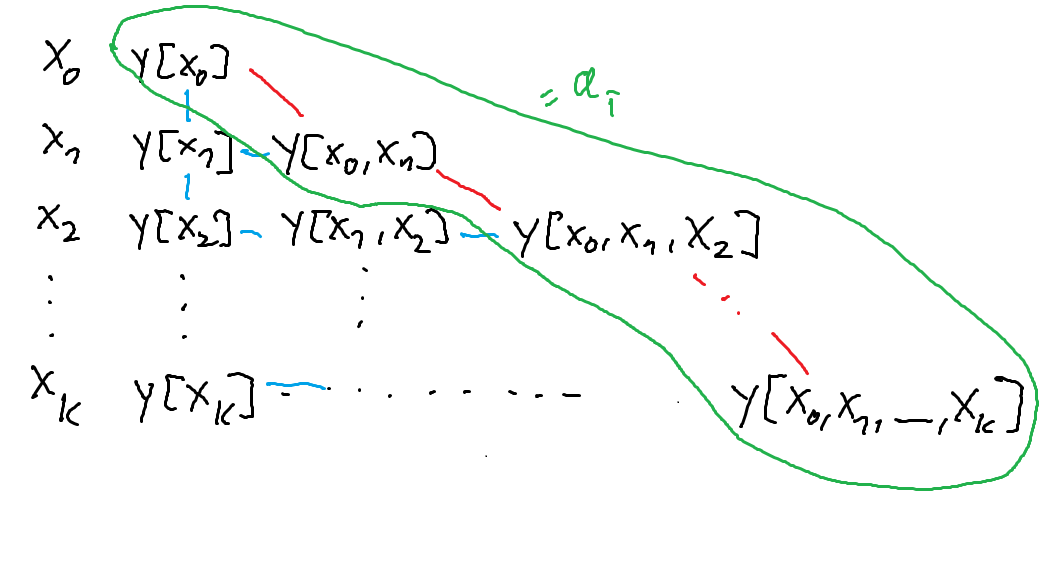
\includegraphics[width=\linewidth]{Bilder/071122_1.png}\\
    \end{center}
\underline{Algorithmus:} berechne $P_{i,j}$:\begin{align*}
    \text{Für }i=0,\dots,n&: P_{i,0} \coloneqq y_i\\
    \text{Für }K\coloneqq 1,\dots,n, \ i=0,\dots,n-k&: P_{i,k} \coloneqq \frac{P_{i+1, k-1}-P_{i,k-1}}{x_{i+k}-x_i}
\end{align*}
\end{question}

\subsection{Auswertung von Polynomen}\hfill\\
Gegenüber der Auswertung von $p(x)=a_0+a_1x+a_2x^2+\dots + a_nx^n$
\[\# multiplikationen:\ n+1+2+\dots + (n-1)=\frac{n(n+1)}{2} \]
Ist die Auswertung der alternativen Darstellung \[p(x)=a_0+x(a_1+x(a_2+x(\dots (a_n-1+xa_n)\dots ))) \]
nach dem "Horner-Schema"\[\begin{cases}
        b_n\coloneqq a_n,& \Rightarrow p(x)=b_0\  \largespace\largespace\# multiplikationen: n\\
    b_k\coloneqq a_k+xb_{k+1},&k=n-1,\dots,0
\end{cases}\]
\begin{enumerate}
    \item deutlich effizienter
    \item oft auch stabiler/besser konditioniert als die Berechnung aller Potenzen
\end{enumerate}
Für die Newton Darstellung: \[
    N_i = \prod_{j=0}^{i-1}(x-x_j) = N_{i-1}\cdot(x-x_{i-1})\]
damit gilt für ein Polynom P die alternative Darstellung\begin{align*}
    p(x) &= \sum_{i=0}^n y[x_0,\dots, x_i]N_i(x) \\
         &= y[x_0] + (x-x_0)(y[x_0, x_1] + (x-x_1)(y[x_0,x_1,x_2]+(x-x_2)(\dots + (x-x_{n-1})(y[x_0,\dots,x_n]))))
\end{align*}
und ein entsprechendes \underline{verallgemeinertes Horner-Schema:} \[
    \begin{cases}
        b_n &\coloneqq y[x_0, \dots, x_n]\\
        b_k &\coloneqq y[x_0, \dots, x_n] + (x-x_k)\cdot b_{k+1}, \midspace k=n-1,\dots,0
    \end{cases}\]
Also $P(x)=b_0$. Dabei ist die Anzahl der Multiplikationen $=n$, somit ist der Aufwand deutlich geringer.
Sind die Stützstellen aufsteigend nach dem Abstand zu $x$ sortiert, dann ist das 
Horner-Schema relativ gut konditioniert.

% hier leon wieder

\subsection{Interpolationsfehler bei der Interpolation einer gegebenen Funktion}\hfill\\
$y_i, \ i=0,\dots,n $ nicht  (willkürlich) vorgegeben, sondern Funktionswerte einer Funktion $f:I\to\R$, mit $I\subset\R$, 
alle $x_i\in I,\ i=0,\dots,n$\\
also $y_i=f(x_i)$. 
\begin{question} Wie groß ist der der Unterschied zwischen $p$ und $f$?\\
\end{question}
Der Unterschied kann mit einem ähnlichen Ausdruck wie Taylor-Restglied abgeschätzt werden:\\

\begin{theorem}
    Sei \[
    \left[\underset{i=0,\dots,n}{\min}x_i,\underset{i=0,\dots,n}{\text{max}}x_i\right] \subseteq I \ \emph{und}\ f\in 
    C^{n+1}(I)
    \]\\
    Dann gibt es zu jedem $x\in I $ ein $ \xi_x\in \left[\underset{i}{\min}(x_i,x),\underset{i}{\text{max}}(x_i,x)\right] $
   \\ mit $\Tilde{I}\coloneqq \left[\underset{i}{\min}(x_i,x),\underset{i}{\text{max}}(x_i,x)\right] $ sodass:\\
    \[
f(x)-p(x)=\frac{f^{(n+1)}(\xi_x)}{(n+1)!}\cdot\prod^n_{j=0}(x-x_j)
    \]
\end{theorem}
\begin{proof}
    Für $x=x_i$, $i\in \set{0,\dots,n}$ ist nichts zu zeigen, da dann \[
        f(x) = p(x), \largespace \prod(x-x_j) = 0\]
    Wir machen einen Ansatz:\[
        g(t)\coloneqq \prod_{j=0}^n(t-x_j)\]
    und \[
        c(x) \coloneqq \frac{f(x) - p(x)}{g(x)}\largespace\text{(eine Konstante abh. von x bzgl. t)}\]
    Setze \[
        F(t) \coloneqq f(t) - p(t) - c(x) \cdot g(t)\]
    Es ist $F(x) = 0$, und \[
        F(x_i) = \underset{=0}{\underbrace{f(x_i) - p(x_i)}} - c(x) \cdot 
        \underset{=0}{\underbrace{g(x_i)}}\]
    \begin{align*}
        &\implies \text{ $F$ hat mindestens $n+2$ Nullstellen in $\tilde{I}$}\\
        &\implies \text{ $F'$ hat mindestens $n+1$ Nullstellen in $\tilde{I}$}\\
        &\implies \text{ $F''$ hat mindestens $n$ Nullstellen in $\tilde{I}$}\\
        \vdots\\
    &\implies \text{ $F^{(n+1)}$ hat mindestens $1$ Nullstelle in $\tilde{I}\eqqcolon \xi_x$ }
    \end{align*}
    und es ist \[
        0 = F^{(n+1)}(\xi_x) = f^{(n+1)}(\xi_x) - \underset{=0, \text{ da } p\in\bbP_n}{\underbrace{P^{(n+1)}(\xi_x)}} - 
        c(x) \cdot \underset{=(n+1)!}{\underbrace{g^{(n+1)}(\xi_x)}}\]
    \[
        \frac{f(x) - p(x)}{g(x)} \cdot (n+1)! = f^{(n+1)}(\xi_x) \implies f(x)-p(x) = \frac{f^{(n+1)}(\xi_x)}{(n+1)!}\cdot 
        \underset{=\prod(x-x_j)}{\underbrace{g(x)}}\]
\end{proof}

% leons schmarn


\begin{corollary}
    Ist $f \in C^\infty(I)$ und es gebe ein $M<\infty$ so, dass \[
    \abs{f^{(n)}(x)} \leq M\midspace \forall n \in \N \text{ und }x\in I 
    \]
    dann Konvergiert die Folge der Interpolationspolynome $p_n\in\bbP_n$ zu $f$ mit beliebigen disjunkten Stützpunkten
    $x_0,\dots,x_n \in I$ auf $I$ gleichmäßig gegen $f$
\end{corollary}
\begin{proof}
    $\forall x\in [a,b]: \abs{f(x)-p(x)} \leq \frac{1}{(n+1)!}\cdot M \cdot (b-a)^{n+1}\to 0$ für $n\to \infty$
\end{proof}

\begin{remark}
    Dies gilt leider nicht für beliebige (auch beliebig glatte) Funktionen
\end{remark}

\begin{remark}
    Satz von Weierstraß sagt aus, dass wir jede \underline{stetige} Funktion $f\in C^0(I)$ beliebig gut gleichmäßig durch 
    Polynome approximieren können. Dies gilt leider \underline{nicht} für die (Lagrange)-Interpolationspolynome
\end{remark}
\begin{example}[Das Runge-Beispiel]\hfill\\
\[f(x)=\frac{1}{1-x^2}\in C^\infty (\R).
\]
Interpolation auf $[-c,+c]$ mit äquidistanten Stützstellen
\[x_i=-c+\frac{2c}{n}i,\ i=0,\dots,n\] 
\begin{center}
    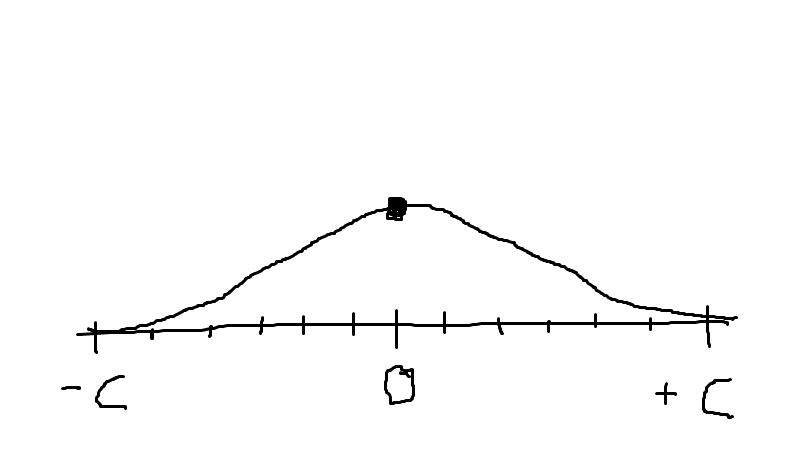
\includegraphics[width=45mm]{../Bilder/x_2.png}\\
\end{center}
Man kann zeigen: ist
\begin{align*}
    c&\leq \frac{e}{2}\implies ||f-p_n||_\infty \to 0 \text{ 
 für } n\to \infty\\
 c&> \frac{e}{2}\implies ||f-p_n||_\infty \to \infty \text{ 
 für } n\to \infty
\end{align*}
warum?\\
\[||f-p||_\infty\coloneqq\underset{x\in [-c,+c]}{\text{max}}|f(x)-p(x)|\] %hier kommt noch ne kleine zeile hin (2. Tafel am 
\[\abs{f^{(n)}(x)} \sim 2^n\cdot n! \cdot \calO{ \abs{x}^{-2-n}}\]
%09.11.)

\end{example}
\begin{example}
    \[
        f(x) = \abs{x}
    \]
    $f$ ist nur in $C^0([-1,+1])$. Äquidistante Stützstellen:\[
    x_i = -1+\frac{2}{n}\cdot i, \largespace i=0,\dots,n
    \]
    Man kann zeigen:\[
    x\neq x_i, \ \text{z.B. } x \text{ irrational, dann }\toInfty P(x) \neq f(x)
    \]
\end{example}
\subsection*{Verhalten gegenüber Störungen in den Daten?}
\begin{example}
    \[I=[-1,1], \largespace x_i=-1+\frac{2}{n}\cdot i, \largespace i=0,\dots,n,\largespace n\text{ gerade }(x_{n/2} = 0)\]
    Wir betrachten Daten\[
    y_i = \begin{cases}
        \eps & i=\frac{n}{2}\\
        0 & \text{sonst}
    \end{cases}
    \] \begin{center}
        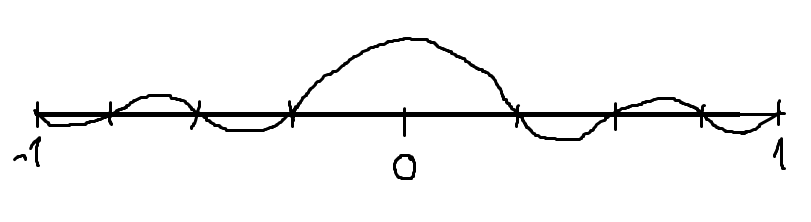
\includegraphics[width=45mm]{../Bilder/x_2_1.png}\\
    \end{center}
    Interpolierende ist \[
    p(x) = \eps\cdot L_{n/2}^{(n)}(x) = \eps\cdot \displaystyle\frac{\dprod_{j\neq \frac{n}{2}}(x-x_j)}{\prod(0-x_i)}
    \]
    Die Faktoren im Produkt sind teilweise > 1,
\end{example}

\begin{question}
    Kann man bei der Interpolation einer Funktion dem Interpolationsfehler  $f-p$ durch geschickte Wahl der Stützstellen 
    kleiner machen?
    \[
f(x)-p(x)=\frac{f^{(n+1)}(\xi_x)}{(n+1)!}\cdot\prod^n_{j=0}(x-x_j)\]\[
W(x)\coloneqq \prod^n_{j=0}(x-x_j)
    \]
\end{question}
Verändern kann man nur den Term 
\[
W(x)= \prod^n_{j=0}(x-x_j).
\]
Man kann zeigen, es gilt spezielle paarweise verschiedene Stützstellen, die $|W(x)|$ gleichmäßig minimieren.\\
\begin{theorem}
    \[\underset{x_0,\dots,x_n\in I}{\min}\underset{x\in I}{\text{max}}\left|\prod^n_{j=0}(x-x_j) \right|=\underset{x\in 
    I}{\text{max}}\left|\prod^n_{j=0}(x-t_j) \right|\]
    mit $x_0,\dots,x_n$ paarweise verschieden und mit den $t_j\in [-1,+1]$ gerade die Nullstellen des "Tschebyscheff-
    Polynoms"\smallspace $T_{n+1}$\\
    
\end{theorem}
\begin{remark}[Optimales $w\in\bbP_{n+1}$?]\hfill\\
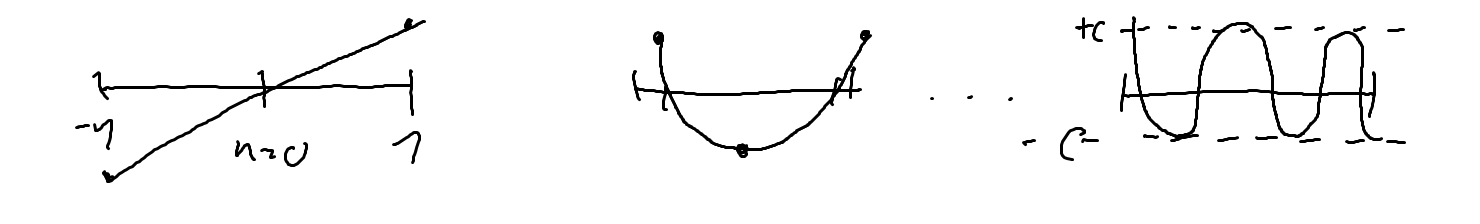
\includegraphics[width=\linewidth]{Bilder/abb1.png}
    Diese Tschebyscheff-Polynome sind für $k\in \N_0$ definiert als \[
    T_k(x)\coloneqq \cos{k\cdot \arccos{x}}
    \]
    mit Nullstellen \[
    t_j=\cos{\frac{2j+1}{2k}\cdot\pi}, \largespace j=0,\dots,k-1
    \]
    Es ist nicht direkt klar, dass $T_k$ überhaupt ein Polynom ist (außer für $k=0,1$):$$\\\begin{cases}
        T_0 &= \cos{0\cdot\arccos(x)} = \cos{0} = 1\\
        T_1 &= \cos{1\cdot\arccos(x)} = x
    \end{cases}$$
    Es gibt folgende 3-Term-Rekursion: \[
    T_0(x)\equiv 1, \ T_1(x) = x, \ T_k(x) = 2x\cdot T_{k-1}(x) - T_{k-2}(x), \largespace k\geq 2
    \]
\end{remark}
Man sieht für das Runge-Beispiel: \\
Auch bei Verwendung der Tschebyscheff-Knoten können für relativ großes $n$, große Fehler am Rand des Intervalles auftreten. 
Abhilfe gelingt bei diesem Beispiel die Verwendung der ''\underline{Tschebyscheff-Knoten zweiter Art}'', das sind gerade 
die Extremstellen des Tschebyscheff-Polynoms: \[
    \Tilde{t_j}=\cos{\frac{j}{n}\cdot \pi},\largespace j=0,\dots,n
\]
\begin{remark}[Kondition/Verhalten bei Störungen:]
    Sowohl bei Tschebyscheff-Knoten erster oder zweiter Art bleibt die Auswirkung einer Störung bei $x=0$ auf dem gesamten
    Intervall $[-1,1]$ beschränkt, im gegensatz zu äquidistanten Knoten. 
\end{remark}

\subsection{Hermite-Interpolation}\hfill\\
Nicht nur Funktionswerte vorgegeben, sondern ggf. auch Ableitungen, evtl. auch höhere.
\begin{definition}
    Die \underline{Hermite-Interpolationsaufgabe}:\\
    \underline{Gegeben:}\\ Stützstellen $x_i, \ i=0,\dots , m$ paarweise verschieden.\\
           \qquad Werte $y_i^{(k)}, \ i=0,\dots , m\ \ k=0,\dots, \mu_i \geq 0$\\
            
    \underline{Gesucht:} Polynom $p\in\bbP_n,\ n\sum_{i=0}^{m}\mu_i$ mit $p^{(k)}(x_i)=y_i^{(x)},\ i=0,\dots,m \ \ 
    k=0,\dots,\mu_i$\\
    Die $x_i$ werden manchmal auch als $\mu_i$-fache Stützstellen bezeichnet.
\end{definition}

\begin{theorem}
    Die Hermite Interpolationsaufgabe ist eindeutig lösbar
\end{theorem}
\begin{proof}
    analog zur Lagrange-Interpolation, ähnliche (nicht im Sinne der Äquivalenzrelation) Matrix zur Vandermonde Matrix
    \begin{align*}
        p(x) &= a_0 + a_1x + \dots + a_nx^n\\
        p'(x) &= a_1+2a_2x+3a_3x^2+\dots+na_nx^{n-1}\\
        \vdots
    \end{align*}
    sind z.B. $p(x_0) = b_0$, $p'(x_0)=c_0$, so gilt für die Matrix \[
        \begin{pmatrix}
            1&x_0&x_0^2&x_0^3&\dots&x_0^n \\
            0&1&2x_0&3x_0^2&\dots&nx_0^{n-1}\\
            \vdots&\vdots&\vdots&\vdots & \vdots&\vdots\\
            0&0&0&0&\dots& 1
        \end{pmatrix}\matrx{
        a_0\\a_1\\ \vdots\\a_n
        }
        = \matrx{b_0\\c_0\\\vdots\\\vdots}
    \]
\end{proof}
\begin{remark}
    Eine ähnliche Aufgabe bei der in Stützstellen eventuell nur \underline{einige} Ableitungen vorgegeben sind, z.B. \[
    p\in\bbP_2: p(x_0) = y_0, p''(x_1) = y_1^{(2)}, p''(x_2)=y_2^{(2)}
    \] 
    ist im allgemeinen \underline{nicht} oder \underline{nicht eindeutig} lösbar
\end{remark}
 Ableitung ist Grenzwert der Differenzenquotienten \[
    \frac{f(x+h) - f(x)}{h} \largespace \text{für }h\to 0
 \]
Ähnlich kann man den Grenzwert der dividierten Differenzen anschauen:\\
Angenommen, die gegebenen Werte $y_i$ sind Werte einer differenzierbaren Funktion $f(x_i) = y_i$, dann ist die erste 
dividierte Differenz gerade \[
    f[x_i, x_j] = \frac{f(x_j) - f(x_i)}{x_j-x_i} 
\]
ist gerade der Differenzenquotient zu $f_1$\\
Für $x_j\to x_i$ konvergiert dann $f[x_j,x_i]\to f'(x_i)\eqqcolon f[x_i,x_i]$\\
So können Hermite Stützstellen mit vorgegebenen Ableitungen als mehrfache Stützstellen aufgefasst werden:\\
Damit können wir das Hermite-Interpolationsverfahten wieder in Newton-Darstellung schreiben, wenn man die dividierten 
Differenzen verallgemeinert:\\
\newcommand{\tx}{\Tilde{x}}
\begin{itemize}
    \item Stützstellen mit (höheren) Ableitungen, also $\mu_i > 0$ werden entsprechend dupliziert, statt $x_i$ wird Folge
    \[\underset{\mu_i + 1-\text{mal}}{\underbrace{x_i, \dots, x_i}}\largespace i=0,\dots, m\]eingefügt, damit bekommt man 
    eine Folge von Stützstellen $\Tilde{x_0}, \Tilde{x_1}, \dots, \Tilde{x_n}$. Für diese werden nun die modifizierten 
    dividierten Differenzen definiert durch \[
    y[\tx_i] \coloneqq y_i^{(0)}, \midspace y[\tx_1, \dots , \tx_{i+k}] \coloneqq \begin{cases}
        y_i^{(k)}\cdot \frac{1}{k!} & \tx_i = \tx_{i+k}\\
        \displaystyle\frac{y[\tx_{i+1}, \dots, \tx_{i+k}] - y[\tx_i, \dots, \tx_{i+k-1}]}{\tx_{i+k} - \tx_i} & \tx_i \neq 
        \tx_{i+k}
    \end{cases}
    \]
    $i$ ist der Original-Index zu $\tx_i = x_i$
\end{itemize}
\begin{theorem}
    Damit hat das Hermite-Interpolationspolynom die Darstellung \[
    p=\sum_{i=0}^n y[\tx_0, \dots, \tx_i] \prod_{j=0}^{i-1}(x-\tx_j)
    \]
\end{theorem}

A8: Stückweise Hermite-Interpolation: Werte $y^{(0)}_i,y_i{(^)}$ auf $I_i=[x_{i-1},x_i]$, $i=1,\dots,m: $
\begin{example}
    Gesucht ist ein $p$ mit $p\in\bbP_4$, $\begin{cases}
        p(0)=-1, \ p'(0)= -2\\
        p(1)=0, \ p'(1)=10, \ p''(1)=40
    \end{cases}$
    $m=1,\ \mu_0=1, \ \mu_1=2$
\end{example}
Direkte Differenzen dazu?\\
\begin{center}
        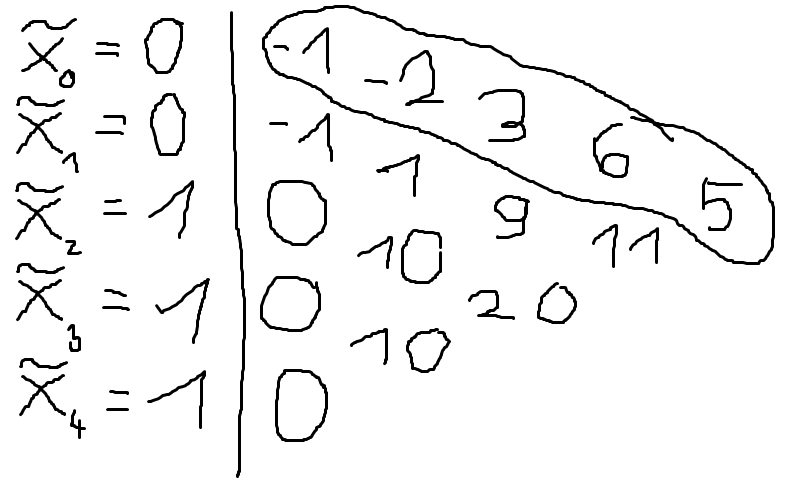
\includegraphics[width=45mm]{../Bilder/x_3.png}\\
\end{center}
\[
\Rightarrow p(x)= -1\ -2\cdot(x-0)\ +3\cdot(x-0)(x-0)\ +6\cdot(x-0)(x-0)(x-1) \ +5(x-0)(x-0)(x-1)(x-1)\]
\[=-1-2x+3x^2+6x^2(x-1)+5x^2(x-1)^2
\]

Ähnlich wie beim Satz über den Fehler der Lagrange-Polynominterpolation kann man zeigen
\begin{theorem}
    Ist \[
    I \coloneqq \set{\min_i(x_i), \max_i(x_i)} \text{ und } f\in C^{(n+1)}(I)
    \]
    Dann gibt es zu jedem $x\in I$ ein $\xi \in I$ so, dass für das Hermite-Interpolationspolynom $p$ zu $f$ gilt\[
    f(x) - p(x) = \frac{1}{(n+1)!}f^{(n+1)}(\xi_x) \cdot \prod_{i=0}^m (x-x_i)^{\mu_i + 1}
    \]
\end{theorem}
Mit der Vorgabe der Ableitungen kann man typicherweise erreichen, dass die oszillationen des interpolierenden Polynoms
zwischen den Stützstellen kleiner werden. Eine andere Möglichkeit/Ansatz dafür:
\subsection{Spline Interpolation}
Bei Polynom-Interpolation erhöht sich der Grad des Polynoms mit Anzahl der Stützstellen/Vorgaben, dies kann dann mit 
höheren $x-$Potenzen zu Oszillationen führen, die nicht gewünscht sind. Ein anderer Ansatz:  Verwende nicht global (auf 
$\R$ bzw. $I$) definierte Polynome, sondern nur \underline{stückweise auf jedem Intervall} (z.B. $[x_{i-1},x_i]$, wenn 
sortiert) und verwende zusätzliche Übergangsbedingungen: Für $\coloneqq x_0<x_1<\dots<x_m=b$ und $I_i=\coloneqq[x_{i-
1},x_i], \ i=1,\dots,n$ ist der entsprechende Funktionsraum dann:\\
\[
    S_{\text{li}}^{(k,r)}[a,b] \coloneqq \set{s\in C^{(r)}[a,b]\colon\  s\vert_{I_i} \in \bbP_k, \ i=1,\dots,n }
\]
($r$-mal stetig diffbar, lokale Polynome vom Grad $\leq k$)

%Hahahhahahahha das Bild 
%WOllen wir einen für die BIlder zuordnen? ALso einer macht die bIlder der rest schreibt ab?
% klingt gut => nehmen wir fynn der hat n tablet

%ich hab keine fettige Haare dAs ist kokosöl \SChwamms
%ich hab aber welche lol cucumber emoji water dropplet emoji \kmujnzhbtgvrfcdsa \frownie
\begin{example}
    Stückweise lineare Interpolation: \[
    S_{\text{li}}^{(1,0)}[a,b] = \set{s\in C^{(0)}[a,b]\colon s\vert_{I_i}\in \bbP_1 }
    \]
    Sind Werte $y_i$ an den Stützstellen $x_i$ vorgegeben, dann ist durch die Vorgabe der Werte in dem Endpunkten jedes 
    Teilintervalls $I_i$ genau ein Polynom $p_i\in\bbP_1$ festgelegt. Stetigkeit über die Intervallgrenzen ergibt sich 
    dadurch, dass sowohl $p_i(x_i)$ und $p_{i+1}(x_i)$ den Gleichen Wert $y_i$ haben. Der Graph der Funktion $s$ ist 
    gerade der Polygonzug mit Eckpunkten $(x_i, y_i),\ i=0,\dots, n$. Auf $I_i$ ist $s\vert_{I_i}$ gereade das 
    Interpolationspolynom zu $(x_{i-1}, y_{i-1}), (x_i, y_i)$. Also haben wir die Fehlerabschätzung für Interpolation einer
    Funktion $f\in C^2[x_{i-1}, x_i]:$\[
        f(x) - p(x) = \frac{1}{2}f''(\xi_x) \cdot \prod_{j=0}^1 \underset{\leq h_i}{\underbrace{(x-x_{i-1 + j})}}
    \] mit $h \coloneqq \max\limits_{i=1, \dots, n}\abs{h_i}$ folgt dann
\end{example}

\begin{corollary}
    Ist $f\in C^2[a,b]$ und $s$ der interpolierende, stückweise lineare Spline, dann gilt:\[
    \underset{x\in [a,b]}{\text{max}} |f(x)-s(x)| \leq \frac{1}{2}\cdot \underset{x\in [a,b]}{\text{max}}|f''(x)|\cdot h^2
    \]
\end{corollary}
\begin{example}
    \[s\in S_h^{(3,1)}[a,b]: \midspace s(x_i) = y_i^{(0)}, s'(x_i)=y_i^{(1)}, \midspace i=0,\dots,n\]
    \begin{center}
        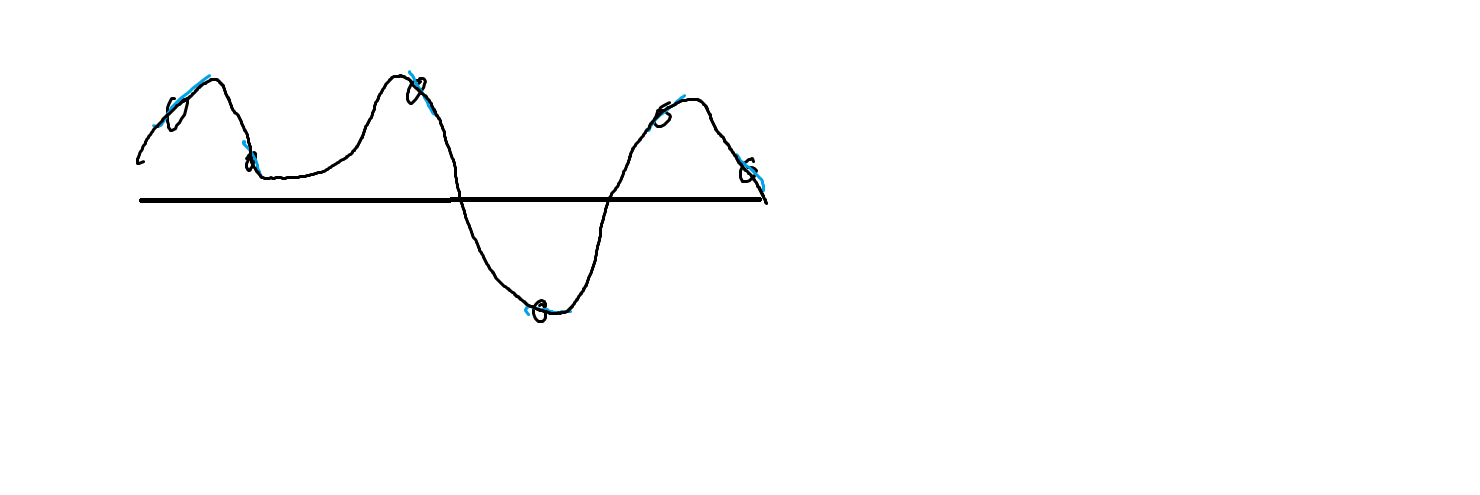
\includegraphics[width=100mm]{Bilder/161122_1.png}
    \end{center}
    $s$ gegeben durch die \underline{stückweise Hermite Interpolation} auf jedem der Teilintervalle.
    Fehlerabschätzung $|f(x)-s(x)|\leq \dots$ siehe Übung A8, für $f\in C^4[a,b]$.\\
\end{example}
''\underline{Kubische Splines}'' : Im gegensatz zu den Hermite-Splines, sollen hier nur \\ die Werte $s(x_i)=y_i,\ 
i=0,\dots, n$ 
vorgegeben werden, dafür soll der Spline insgesammt glatter sein:\[
s\in S_h^{(3,2)}[a,b]=\left\{s\in C^2[a,b]\colon s\vert_{I_i}\in \bbP_3 , \ i=1,\dots, n\right\}\]
\begin{question}[Kann das überhaupt Funktionieren?]\hfill\\
    $S\vert{I_i}\in \bbP_3$, $s'\vert_{I_i}\in\bbP_2$, $s''\vert_{I_i}\in\bbP_1$, $s''\vert_{I_i}\in\bbP_0$, konstant.
    Es gilt \[
        s \in C^2[a,b] \implies s'' \text{ ist Polygonzug auf }[a,b]
    \]
    Wieviel Bedingungen ergeben sich? Wieviel Freiheitsgerade gibt es?
    \begin{align*}
        n &\text{ Teilintervalle } I_i,\ s\vert_{I_i}=P_i\in\bbP_3 \to \ &&4\cdot n\ \text{Koeffizienten ''frei''}\\
    s(x_i^-)&=y_i,\ i=0\dots,n \ &&n+1\quad \text{Bedingungen}\\
        s(x_i^-)&=s(x_i^+),\ i=1\dots,n-1 \qquad &&n-1 \\
        s'(x_i^-)&=s'(x_i^-),  \ &&n-1 \\
        s''(x_i^-)&=s''(x_i^+),  \ &&n-1 \quad 4n-2 \text{ Bedingungen}
    \end{align*}
    Wir haben also weniger Bedingungen als Koeffizienten, die Bediungngen sollten demnach zu erfüllen sein. Um die 
    Eindeutigkeit zu bekommen sind eventuell noch 2 Bedingungen zusätzlich zu stellen, z.B.:
  \begin{align*}
      \text{Steigung in }a,b:\hspace{10em} & s'(x_0), \midspace s'(x_n)\\
      \text{Krümmung in }a,b:\hspace{10em}& s''(x_0), \midspace s''(x_n)\\
      \text{Periodizität}:\hspace{10em} & s(x_0) = s(x_n), \midspace s'(x_0) = s'(x_n),\\ & s''(x_0) = s''(x_n), \midspace 
      y_0 = y_n
  \end{align*}
  Das Wort ''Spline'' bezeichnet (englisch) eine dünne, biegsame Latte, z.B. Konstruktion der Form eines Schiffrumpfs. 
  Latte versucht (unter der Vorgabe der festen Punkte) ihre elastische Energie zu minimieren. Das entspricht der \underline{
  Minimierung der Gesamtkrümmung}. Krümmung eines Graphen $(x,f(x))$:\[
    \kappa(x,f(x)) = \frac{f''(x)}{\sqrt{1+\abs{f'(x)}^2}^{\frac{3}{2}}}
  \]
  Für die Gesamtenergie gilt\[
    E(f) \coloneqq \int_a^b \abs{\kappa(x,f(x))}^2 \cdot \sqrt{1+f'^2} dx \approx \int_a^b \abs{f''(x)}^2 dx \text{ (nach 
    Linearisierung)}
  \]
  Versucht man, unter allen glatten Funktionen, die in den $x_i$ interpolieren, diese Energie zu minimieren, bekommt man 
  gerade das kubische Spline
\end{question}

\begin{theorem}
    \(a=x_0<x_1<\dots<x_n=b, y_i \in \R , \ i=0,\dots,n\)\\
    \(A\coloneqq \{ f\in C^2[a,b]\colon f(x_i)=y_i, \ i=0,\dots,n\}\)
    Dann gibt es genau eine Lösung $s\in A$ mit \[
        E(s) \leq E(f)\largespace \forall f\in A
    \] mit \[
        E(f) \coloneqq \int_a^b (f''(x))^2 dx
    \]
    und dieses \(s\in S^{(3,2)}_h[a,b]\) mit $s''(a)=s''(b)=0$, $s$ ist ein ''\underline{natürlicher Spline}''
    
\end{theorem}
\begin{proof}
    Seien $f,s\in A$, und $s\in S^{(3,2)}_h[a,b]$. Zu zeigen:\[
        E(s) \leq E(f)
    \]
    Wir betrachten $f-s$: \begin{align*}
        E(f-s) &= \int_a^b (f''(x) - s''(x))^2 dx\\
               &= \int_a^b (f'')^2 dx  - 2 \int_a^b f''s'' dx + \int_a^b (s'')^2 dx\\
              \text{\PHpedestrian} &= \int_a^b (f'')^2 dx - 2 \int_a^b(f'' - s'')s'' dx - \int_a^b (s'')^2 dx
    \end{align*}
    Mittlerer Term = 0 ?!?!?!?!?!?!?\begin{align*}
        \int_a^b(f'' - s'') s'' dx &= \dsum_{i=1}^n \int_{I_i}(f'' - s'')\underset{\in \bbP_3 \subset C^\infty}
        {\underbrace{s''\vert_{I_i}}} dx\\
        &= \dsum_{i=1}^n\left([f'-s']_x{i-1}^{x_i} - \underset{=s'''\vert_{I_i} \int_{I_i}(f-s)'dx}{\underbrace{\int_{I_i}
        (f'-s')\underset{\text{konstant auf $I_i$}}
        {\underbrace{s'''}} dx}}\right)\\
        &=\left((f'-s')\underset{=0}{s''}\right)(x_n)-\left((f'-s')\underset{=0}{s''}\right)=0, \\ &\Rightarrow 
        \text{\PHpedestrian} \Rightarrow 0\leq E(f)-E(s) \Rightarrow E(s)\leq E(f)
    \end{align*}
    Zur \underline{Eindeutigkeit:}\\
   \newcommand{\Ts}{\Tilde{s}}
    angenommen, $s,\Tilde{s} \in S^{(3,2)}_h[a,b]$ beides Lösungen. Zu zeigen: 
        $s=\Tilde{s}$
    Damit ist 
    \begin{align*}
        E(s-\Tilde{s})= E(s)-E(\Tilde{s})=0\text{ (wie oben) } &\Rightarrow \int_a^b(s''-\Ts'')^2(x)dx = 0 \\
        &\Rightarrow (s-\Ts)''(x)\ \forall x\in [a,b]\\
        &\rightarrow (s-\Ts)\in\bbP_1[a,b], \ s(x)-\Ts(x)=a_0+a_1x\\
        &\ \ s(x_i)=\Ts(x_i),\ i=0,\dots,n \\
        &\Rightarrow s(x)-\Ts(x)\equiv 0
    \end{align*} 
    Zur \underline{Existenz:}\\
    mit linearer Algebra: alle Bedingungen sind \underline{lineare} Gleicuhngen in den Koeffizienten $(a_j{(i)},
    \ i=1,\dots,n, \ j=0,1,2,3)$\[
        \vert_{I_i}= a_0^{(i)} + a_{0}^{(i)}x + a_{2}^{(i)}x^2 + a_3^{(i)}x^3
    \]
    Also haben wir $4n$ Bedingungen (linear!) für $4n$ Unbekannte und somit ein quadratisches LGS mit linearer Abb. A.
    Aus der Eindeutigkeit folgt, dass $\Kern{A} = \set{0}$ und $\dim\Bild{A} = 4n$. Dementsprechend haben wir eine 
    eindeutige Lösung für jede rechte Seite 
\end{proof}

\begin{proof} (Ein Konstruktiver Existenzbeweis)\hfill\\
Wie oben: \[
s\vert_{I_i}\in\bbP_3 \leadsto s''\vert_{I_i}\in\bbP_1,\ s'' \text{ stetig }\leadsto s''\text{ Polygonzug}.
\]
Sei 
\begin{align*}
    M_i&\coloneqq s''(x_i),\ i=0,\dots, n \\
    \implies s''\vert_{I_i}(x)&=\frac{M_{i-1}(x_i-x)+M_{i}(x-x_{i-1})}{x_i-x_{i-1}}\\
    \implies s''\vert_{I_i}(x)&=\dfrac{1}{h_i}(M_{i-1}(x_i-x)+M_{i}(x-x_{i-1}))\\
    \implies s'\vert_{I_i}(x)&= \frac{1}{h_i}(M_{i-1}\frac{(x_i-x)^2}{2}+M_{i}\frac{(x-x_{i-1})^2}{2}) + c_i , \ c_i\in\R \\
    \implies s\vert_{I_i}(x) &= \frac{1}{h_i}(M_{i-1}\frac{(x_i-x)^3}{6}+M_{i}\frac{(x-x_{i-1})^3}{6}) +c_i(x-x_{i-1})+d_i, \ 
    d_i\in\R
\end{align*}

Stetigkeit in \(x_i,\ i=1,\dots,n-1 \implies \) Bedingungen für \((\mu_i, c_i, d-i)\) 

\end{proof}

Stetigkeit von $s'$ in $x_i$ bedeutet\[
    s_i'(x_i) = s_{i+1}'(x_i) : M_i \frac{h_i}{2} + c_i = -M_i\frac{h_{i+1}}{2} + c_{i+1}\largespace \left(\text{\PHchild}
    \right)\]
    Interpolation: \begin{align*}
        s(x_i) = y_i &\implies y_{i-1} = \frac{1}{6}h_i^2\cdot M_{i-1}+ d_i, 
        \midspace y_i = \frac{1}{6}h_i^2\cdot M_i+c_ih_i+d_i\\
        &\implies \frac{y_i-y_{i-1}}{h_i} = \frac{h_i}{6}(M_i - M_{i-1}) + c_i\\
        &\implies c_i = y[x_{i-1}, x_i] - \frac{1}{6}h_i(M_i- M_{i-1}), \midspace d_i = y_{i-1}-\frac{1}{6}h_i^2M_{i-1}
    \end{align*}
    in $\left(\text{\PHchild}\right)$ einsetzen.

\begin{align*}
    \frac{1}{2}h_iM_i-\frac{1}{6}h_i(M_i-M_{i-1})+y[x_{i-1},x_i]&=
    -\frac{1}{2}h_{i+1}M_i-\frac{1}{6}h_{i+1}(M_{i+1}-M_{i})+y[x_{i},x_{i+1}] \\
    h_iM_{i-1}+2(h_i+h_{i+1})M_i+h_{i+1}M_{i+1} &= 6(y[x_{i},x_{i+1}]-y[x_{i-1},x_i]) \\
    \intertext{Setze \(\mu_i = \frac{h_i}{h_i+h_{i+1}}\) und \(\lambda_i=\frac{h_{i+1}}{h_i+h_{i+1}}\)}
    \mu_iM_{i+1}+2M_i+\lambda_iM_{i+1}&=y[x_{i-1},x_i,x_{i+1}]
\end{align*}

Dies ergibt ein lineares Gleichungssystem für die $M_i, i=1,\dots,n-1$ ($M_0 = 0, M_n = 0$, da natürlicher Spline)
\[
    \matrx{2&J_1&\ &\dots\\\mu_2&2&J_2& \ \\\ &\ddots&\ddots&J_{n-2}\\\ & \ & \mu_{n-1}&2}\cdot \matrx{
        M_1\\M_2\\\vdots\\M_{n-1}} = \matrx{6y[x_0,x_1,x_2]\\ 6y[x_1,x_2,x_3]\\\vdots\\6y[x_{n-1},x_{n-1},x_n]}
    \]
Die Matrix des linearen Gleichungssystems ist ''strikt diagonaldominant''. Also gibt es eine 
eindeutige Lösung\begin{definition}
    Eine Matrix $A\in \R^{m\times m}$ oder $A\in \C^{m\times m}$ heißt \begin{itemize}\item''\underline{strikt 
    diagonaldominant}'',
    wenn \[
        \forall i=1,\dots,m: \midspace\abs{a_{ii}} > \dsum_{\substack{j=1\\j\neq i}}^m \abs{a_{ij}}\]
    \item''\underline{schwach diagonaldominant}'', wenn \[
        \forall i=1,\dots,m: \midspace\abs{a_{ii}} \geq \dsum_{\substack{j=1\\j\neq i}}^m\abs{a_{ij}}\]
    und für \underline{mindestens} ein $i$ es ''$>$'' ist.
    \end{itemize}
\end{definition}
\begin{lemma}
    Ist $A$ strikt diagonaldominant, so gilt \[
        \forall z\in\R^n(\C^n): \dabs{Az}_{\max} \geq c\cdot \dabs{z}_{\max}\]
    mit \[
        c = \min_i\left(a_{ii} - \dsum_{\substack{j=1\\j\neq i}}\abs{a_{ij}}\right)\]
\end{lemma}

\begin{theorem}
    \(a=x_0<x_1<\dots<x_n=b\) Die Interpolationsprobleme mit kubischen Splines:
    \begin{enumerate}[i)]
        \item Für ''\underline{natürliche Splines}'' \(s(x_i)=f_i, i=0,\dots,n,\ M_0=M_n=0\) bzw. \(s''(x_0)=s''(x_n)=0\)
        \item Für ''\underline{vollständige Splines}'' \(s(x_i)=f_i, i=0,\dots,n,\ s'(x_0)=f'(x_0),\ s'(x_n)=f'(x_n)\) 
        \item Für ''\underline{periodische Splines}'' \(s(x_i)=f_i, i=0,\dots,n,\ \) mit \(f_0=f_n,\ s'(x_0)=s'(x_n),\ 
        s''(x_0)=s''(x_n)\)
        \item Für ''\underline{not-a-Knot-Splines}'' \(s(x_i)=f_i, i=0,\dots,n,\) \(s'''\) stetig in \(x_1\) und 
        \(x_{n-1}\) \(\Rightarrow\) \(s\vert_{I_1\cup I_2}\in\bbP_3,\ S\vert_{I_{n-1}\cup I_n}\in\bbP_3\)
    \end{enumerate}
    sind stets \underline{eindeutig lösbar}.\\
    \textit{(kein neuer Beweis, ähnliche Beweise für ii), iii) iv))}
\end{theorem}

\begin{question}[Fehler bei der Splineinterpolation?]\hfill\\
    \begin{reminder} Hermite Interpolation:\[
        \dabs{f-s}_{\max}\leq \frac{1}{4!}h^4\dabs{f^{(4)}}_{\max}\]    
    \end{reminder}
\end{question}
\begin{theorem}
    $a = x_0 < x_1 < \dots, < x_n = b$ und $f\in C^4[a,b],$ $h\coloneqq \max\limits_{\igb{i}{1}{n}}(x_i - x_{i-1})$
    Dann ist für den interpolierenden kubischen Spline \[
        \dabs{f-s}_{\max[a,b]} \leq h^4\dabs{f^{(4)}}_{\max[a,b]}\]
\end{theorem}
\begin{proof}
    $(f-s)(x_i) = 0$. Dann ist auf jeden Teilintervall $I_i$ das Polynom $p_0\equiv0$ die lineare Interpolierende
    zu $f-s$. Die Interpolations-Fehlerabschätzung liefert\[
        \dabs{(f-s) - p_0}_{\max I_i} = \dabs{f-s}_{\max I_i} \leq \frac{1}{2}h_i^2\dabs{(f-s)''}_{\max I_i} = \frac{1}
        {2}h_i^2\dabs{f''-s''}_{\max I_i}\]
    Sei nun $p_i\in \bbP_1$ das Polynom, das $f''(x_{i-1})$ und $f''(x_i)$ interpoliert. Dann ist \begin{align*}
        \dabs{f'' - s''}_{\max I_i} &\leq \dabs{f'' - p_i}_{\max I_i} + \dabs{p_i - s''}_{\max I_i}\\
                                    &\leq \frac{1}{2}h_i^2\dabs{f^{(4)}}_{\max I_i} + \max\limits_{j = i-1, i}\abs{f''(x_j) 
                                    - s''(x_j)}
    \end{align*}

Siehe oben: 
\\
\textit{Die Matrix A ist auf dem Tafelbild ... zu sehen!!} \frownie 
\\
\(
A=\begin{pmatrix}
    2 & \lambda_i & \ \\
    \mu_i & \ddots & \ddots \\
    \ & \ddots & 2
\end{pmatrix} \implies ||Az|| \geq c||z||_{\text{max}} \) mit \(c=1\), also \(||z||_{\text{max}}\leq||Az||_{\text{max}}\)\\
mit \(z_i= f''(x_i)-M_i\) folgt \[\max\limits_{i}|f''(x_i)-M_i|\leq \max\limits_{i}|\mu_if''(x_{i-i})+2f''(x_i)+
\lambda_if''(x_{i+1})|\]
\end{proof}

% Lennart muss die letzte Tafel noch machen. hat er aber noch nicht lol. Kommt auch noch in den Beweis mit rein!!! jaja

\section{Trigonometrische Interpolation}\hfill\\
Ein Ansatz zur Interpolation von periodischen Signalen/Daten mit $\sin{}$/$\cos{}$-Funktionen z.B.bei akustischen 
Signalen.\\
\subsection{Zum Hintergrund} ''\underline{Fourier-Transformation}'': auch für nicht periodische Funktionen:
\[
f\colon \R \to \C \colon \mathcal{F}(f)(y)=\coloneqq \frac{1}{\sqrt{2\pi}}\int_\R f(x)e^{-ixy} dx
\]
mit $i^2=-1$
\[
e^{a+ib}\coloneqq e^a\cdot(\cos{b}+i\sin{b})
\]
Dann ist
\[
f(x)=\frac{1}{\sqrt{2\pi}}\int_\R F(x)e^{-ixy} dx
\]
z.B. für alle $f\in L^1 (\R)$\\
\subsection{Fourier-Reihen}
Für \underline{periodische} Funktionen, z.B. \(f\colon\R\to\C\) \(2\pi\)-periodisch, also \(f(x+2\pi)=f(x)\quad \forall x \in \R\)
Damit\[
f(x)=\frac{a_0}{2}+\sum^\infty_{k=1}a_k\cos{kx}+\sin{kx}
\]
bzw.\[
f(x)=\sum_{k\in\Z}c_k\cdot e^{ikx}
\]
mit\[
c_k=\frac{1}{2\pi}\int_{-\pi}^\pi f(s)\cdot e^{-iks}ds\in \C 
\]
Damit ist\[
a_k=c_k+c_{-k},\ b_k=i(c_k-c_{-k})
\]
bzw.
\begin{align*}
  a_k&=\frac{1}{\pi}\int_{-\pi}^\pi f(s)\cdot \cos{ks}ds \\
  b_k&=\frac{1}{\pi}\int_{-\pi}^\pi f(s)\cdot \sin{ks}ds
\end{align*}
Konvergenz der Fourierreihe für beliebige \(L^1\) oder \(L^2\)-Funktionen auf \((-\pi,\pi)\), bzw. stetige, periodishce 
Funktionen auf \([-\pi,\pi]\)\\
Abgebrochene Reihe/Partialsummen $\to$ Approximation der Funktion $f$.
\subsection{Diskrete Fourier-Transformation}
Gegeben Werte \(a_k, \igb{k}{0}{n-1}\) an Punkten \(x_k = k\frac{2\pi}{n}\) Mit den Koeffizienten \[
    \hat{a_j} = \dsum_{k=0}^{n-1}a_k\cdot e^{\displaystyle-i\cdot j \cdot k \cdot\frac{2\pi}{n}}
\]
ist dann \[
    a_k = \frac{1}{n}\dsum_{j=0}^{n-1}\displaystyle{\hat{a_j}\cdot e^{\displaystyle ijk\frac{2\pi}{n}}} = 
    \frac{1}{n}\dsum_{j=0}^{n-1} \hat{a_j}\cdot\left(\cos{jk\frac{2\pi}{n}}+ i\sin{jk\frac{2\pi}{n}}\right)
\]
Diskrete Fourier Transformation lässt sich auf Polynom-Interpolation zurückführen mit \[
    w\coloneqq e^{ix}, \largespace w_k \coloneqq e^{ixk} = e^{i2\pi \frac{k}{n} }
\]
\begin{center}
    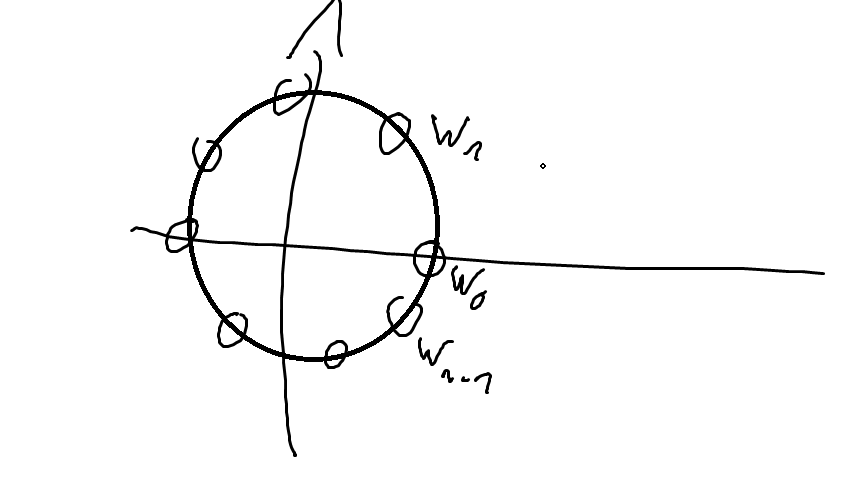
\includegraphics[width=\linewidth]{Bilder/231122_1.png}
\end{center}
Dann ist DFT gerade \[
    t_n(x) = \dsum_{j=0}^{n-1}\frac{\hat{a_j}}{n}\cdot e^{ijx} = \dsum_{j=0}^{n-1}\frac{\hat{a_j}}{n}w^j = p(w), 
    \largespace \text{mit } p\in \bbP_{n-1}
\]
Polynominterpolation wie in 2.1 - 2.3 geht ganz genau so f+r Komplexwertige Polynome \(p\in\bbP_n[\C]\). Daraus folgt
die Existenz und Eindeutigkeit eines \underline{interpolierenden Polynoms} für Werte \(a_k\) an Punkten \(w_k, \ \igb{k}
{0}{n-1}\). Berechnung der Fourierkoeffizienten \(\hat{a_j}\) nicht über Polynom-Methode, sondern entsprechend obiger Formel,
bzw. über ''\underline{Fast Fourier Transformation}'', mit Aufwand \(\calO{n\cdot\log n}\) statt\(\calO{n^2}\). \\
Anwendung: z.B. MP3-Kompression von Audio-Dateien.
\end{document}